\section{Selecting the method by complete reduction time}
\label{sec:refined-time}
The target integrals and required master basis determine which seed regions can support a reduction. A region that excludes a required master can cause an unsuccessful attempt and a repeat calculation. We therefore include basis information in both the model inputs and the candidate settings, and train the model to minimize the complete time after recovery. Kira's subsector cutoff admits numerator ranks zero and one, and can also admit a master through an explicitly assigned sector limit~\cite{Kira3}. Two candidates use this condition to retain the required masters with the least enlargement of that cutoff. The selector compares their measured cost with seven other settings. Exact formulas and independent-loop factorization precede prediction, and Kira computes the coefficients for each remaining native block.

\subsection{Training and integration}
The nine settings include the original native bounds, six conservative basis-compatible candidates, and two candidates with the tighter cutoff condition. The new pair uses the ordinary or increased numerator-rank bound. Appendix~\ref{app:refined-time} derives the new condition from Kira's cutoff, while Appendix~\ref{app:total-time} gives the shared timing objective and structural inputs. Every candidate retains the exact basis check and recovery code. The exact formulas retain their assumptions from Appendix~\ref{app:blocks13}.

The model receives the 44 structural inputs used above and seven summaries of the supplied master basis. These additional inputs describe its size, positive-power bounds, numerator ranks, dots, truncation limit, and differences from the target bounds. No family name or parameter-profile identifier enters the features. Each candidate action is timed through process completion and an independent exact coefficient check, including failed attempts and recovery. We use one repetition for each training action and two for each validation action. Unverified outcomes receive a declared training penalty and remain in the evidence.

The collection contains 31 training requests and 20 validation requests, with separate rational parameter profiles and symbolic dimension. It covers vacuum, two-point, and scattering structures through three loops. Pentagon requests are absent from both sets. We fit trees with maximum depths one through five and minimum leaf sizes two, four, or seven, using either one tree or sixteen trees. The split objective minimizes elapsed reduction cost. Validation retains the fixed setting because the fitted candidates do not meet the declared improvement threshold. The deployed application therefore performs no tree prediction. It compares the selected method with the fastest fixed candidate before enabling prediction. The selected fixed action is a truncation with the tighter basis condition and increased rank. The validation totals are 42.586 seconds for the selected application, 45.714 for native choices, and 42.586 for the fixed candidate. The model changes the best fixed action on 0 of the 20 validation requests. These are model-selection measurements.

The application loads model weights and computes predictions only for a block that needs native algebra. An exact formula therefore incurs no model prediction. Identical independent blocks share one reduction within the request, and the resulting product remains factored. When prediction is enabled, a structural-range check sends inputs outside the training ranges to native settings. The selector also retains native settings when no checked master basis is available. These rules avoid unsupported learned choices; they do not establish that an unseen integral will reduce quickly.

\subsection{Reserved comparison}
We freeze the weights and decision rules before using the new test profiles. Every request compares the learned application, native choices, a validation-selected fixed choice, and the previously published application. The first three methods use identical exact formulas, basis checks, and recovery code. The native control uses the original seed bounds; the learned and fixed methods choose from the same nine candidates. The comparison with the best fixed choice therefore measures the added request-dependent decision. The previous application also differs in basis-aware seeding, model implementation, and output handling, so that comparison measures the complete update.

The test contains 65 requests. It includes new target shapes and parameter values, the held-out pentagon structure, independent products through thirteen loops, the two specified analytic families at thirteen loops, and the previously difficult three-loop ladder. Each method runs three times in rotated order on the same worker. A method that fails its first exact check receives no further repetitions for that request. The learned application completes all three checks on 64 requests; Table~\ref{tab:refined-time} retains the other outcomes.

On 64 matched requests, the application uses 209.217 seconds against 228.710 seconds for the previous application, or 8.5\% less time. The time ratio is 0.915, with repetition interval $[0.864,0.918]$. On 64 matched requests, the application uses 209.217 seconds against 213.807 seconds for native bounds, or 2.1\% less time. The time ratio is 0.979, with repetition interval $[0.962,0.990]$. On 64 matched requests, the application uses 209.217 seconds against 210.378 seconds for the best fixed setting, or 0.6\% less time. The time ratio is 0.994, with repetition interval $[0.984,1.008]$. Validation leaves prediction off. These measurements describe the fixed workflow and do not establish an added gain from the fitted forest.

\begin{table}[!htbp]\centering\small
\caption{Complete-time comparison on the same requested workload. The first-pass column includes one timed attempt for every request, including unverified outcomes. Each ratio divides the summed request medians for the learned method by those for the listed method, using only their matched exact completions.}
\label{tab:refined-time}
\begin{tabular}{@{}lrrrr@{}}\toprule
Method & Verified requests & First pass (s) & Learned/method & Failed calls\\\midrule
Previous application & 64/65 & 343.848 & 0.915 & 36\\
Native choices & 64/65 & 286.701 & 0.979 & 5\\
Fixed choice & 64/65 & 283.179 & 0.994 & 2\\
Learned selector & 64/65 & 280.860 & 1.000 & 2\\
\bottomrule\end{tabular}
\end{table}
\begin{figure}[!htbp]\centering
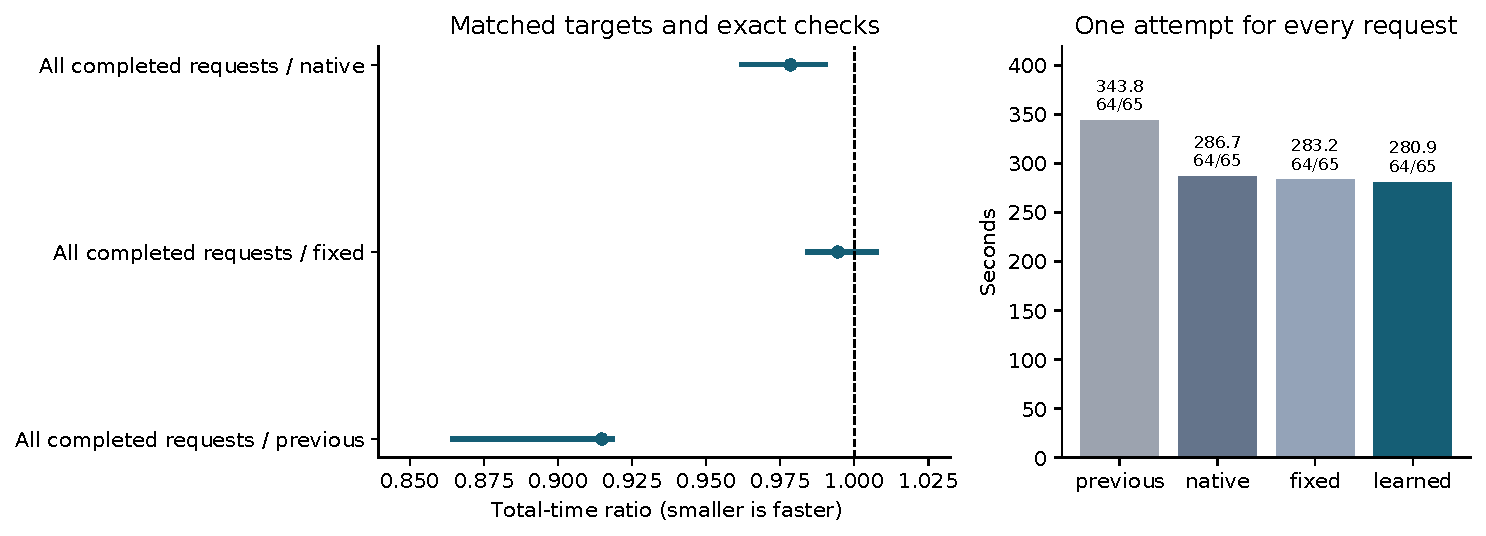
\includegraphics[width=\linewidth]{paper_figures/refined_time_selection.pdf}
\caption{The left panel separates the complete application change from the added learned choice. Each point uses completed matched requests; bars show variation from resampling the three repetitions, and the dashed line marks equal time. The right panel includes one attempt for every requested calculation. Its labels give elapsed seconds and verified coverage, so an unfinished request cannot appear as a successful speedup.}
\label{fig:refined-time}
\end{figure}
\begin{table}[!htbp]\centering\small
\caption{Use of the selector in each physical domain. The pentagon row is a subset of coupled requests. The ratio uses only matched requests that invoke the model, with the best fixed candidate as control. A dash means that no such comparison exists.}
\label{tab:refined-domains}
\begin{tabularx}{\linewidth}{@{}Yrrrr@{}}\toprule
Domain & Requested & Verified & Use ML & ML/fixed\\\midrule
Coupled families & 29 & 28 & 0 & --\\
Independent products & 34 & 34 & 0 & --\\
Analytic formulas & 2 & 2 & 0 & --\\
Pentagon subset & 2 & 2 & 0 & --\\
\bottomrule\end{tabularx}\end{table}

Across every timed attempt, the learned application uses 701.490 seconds, native choices use 715.190, the fixed choice uses 703.361, and the previous application uses 814.261. These totals include all recorded repetitions and failures. Independent reference preparation takes 440.803 seconds outside the application timers. The existing checked master-basis preparation and training-label collection also precede deployment. The 639 training and validation action measurements use 1509.683 seconds in total, before independent reference preparation and 8.568 seconds of model fitting. The supplied-basis comparison therefore measures subsequent reductions, rather than a complete first-use calculation with unknown masters.

The high-loop results remain specific to the defined analytic families and products of small independent blocks. The coupled native tests reach three loops. No result establishes a globally minimum reduction time or complete coverage of arbitrary thirteen-loop scattering. The earlier seed and equation models retain their separate measured domains; the present selector keeps native equation and row choices, and we do not multiply savings from separate experiments.
